\section{Risultati Ottenuti}

\subsection{Nessun intervento}
Il seguente grafico \ref{fig:abm_no_intervent} mostra l'andamento delle curve del modello
quando questo viene eseguito senza alcuna tipologia di intervento. Questo andamento e' mostrato 
in maniera cumulativa rispetto all'andamento dei singoli agenti, i quali possono mostrare comportamenti 
differenti tra loro.

\begin{minipage}{\linewidth}
	\centering
	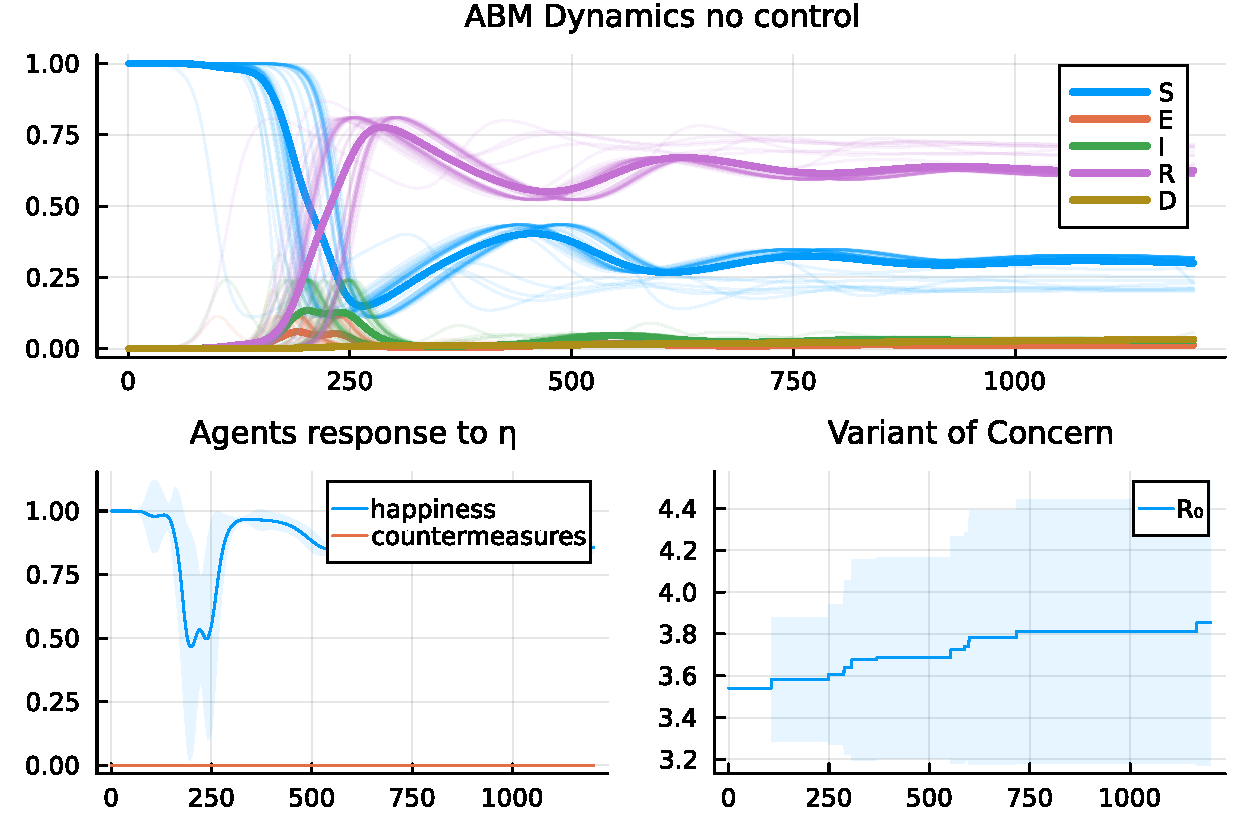
\includegraphics[width=\textwidth]{img/SocialNetworkABM_NO_CONTROL.pdf}
	\captionof{figure}{Grafico cumulativo del modello senza senza alcun tipo di intervento}
	\label{fig:abm_no_intervent}
\end{minipage}

Complessivamente l'andamento del modello e' similare all'andamento standard di un modello di tipo  
SEIR, con qualche variazione dipendente dai fattori di stocasticita' intrisechi del modello; che in questo
caso non sono troppo presenti. Il grafico mostra le traiettorie piu' comuni delle curve cumulate del modello, 
dove vengono messe in evidenza i percorsi piu' utilizzati. 

Come e' possibile notare, il numero di individui suscettibili crolla drasticamente
per via della diffusione rapida e simil esponenziale che ha il virus. Questa viene emulata
dall'altrettanto rapida crescita di individui guariti (recovered) che pero', per via
di come e' stato definita la condizione di guariti, non sono immuni alle varianti del virus, permettendo 
di modellare una possibile ciclicita' dell'epidemia data dalla perdita di immunita' della popolazione. 
Queste proprieta' contribuiscono ad un andamento ciclico delle curve. Si puo' notare come 
la curva associata all'andamento degli individui nella classe \emph{D} abbia una crescita lineare, 
seppur non troppo evidente.

A seguire si puo' osservare come la curva associata alla variabile di happiness del modello,
valore che serve per bilanciare la durezza delle misure di controllo per evitare 
di cadere in un ciclo funzionale ma insostenibile, mostra un comportamento alquanto bizzarro.
Questo e' dovuto principalmente a come viene definita la funzione di controllo della felicita' \ref{fig:happiness}.
Si osserva inoltre che la curva tende ad un \emph{plateau} passato il periodo della "prima ondata".

\begin{minipage}{\linewidth}
	\centering
	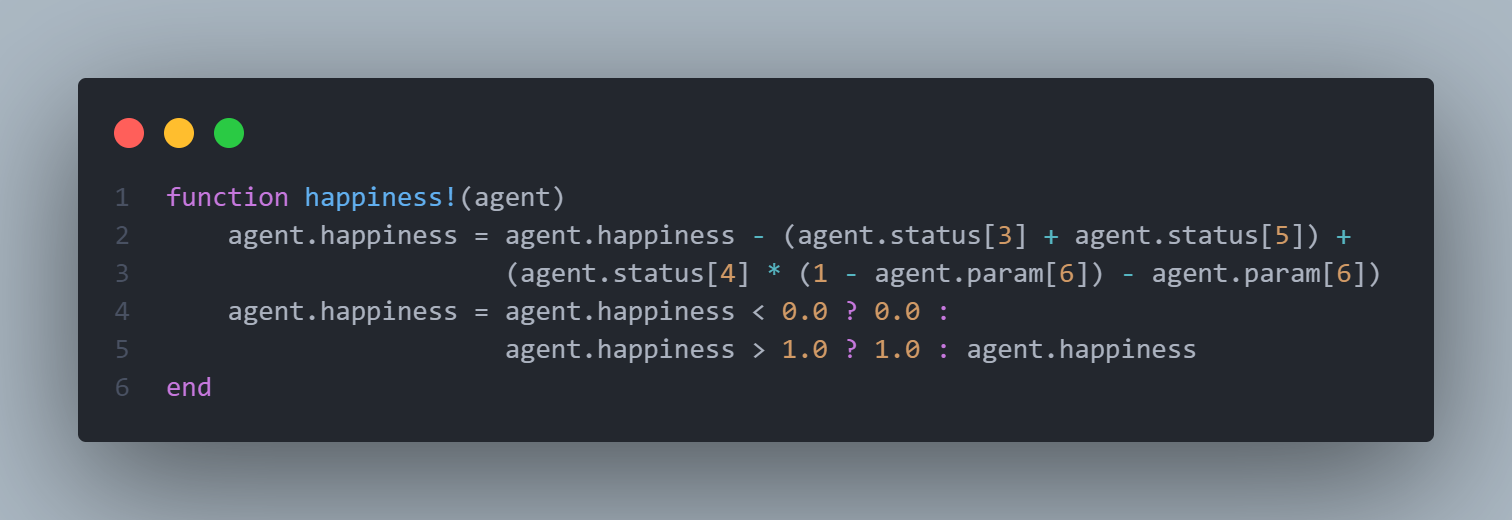
\includegraphics[width=\textwidth]{img/happiness.png}
	\captionof{figure}{Definizione funzione di happiness}
	\label{fig:happiness}
\end{minipage}

Questo comportamento principalmente irrealistico e associato alla definizione che e' stato fatto della 
funzione \textbf{happiness} \ref{fig:happiness}. Il comportamento di questa curva non e' completamente 
realistico, e' comunque utilizzabile per lo scopo di mantenere sotto controllo le contromisure $\eta$.

\begin{minipage}{\linewidth}
	\centering
	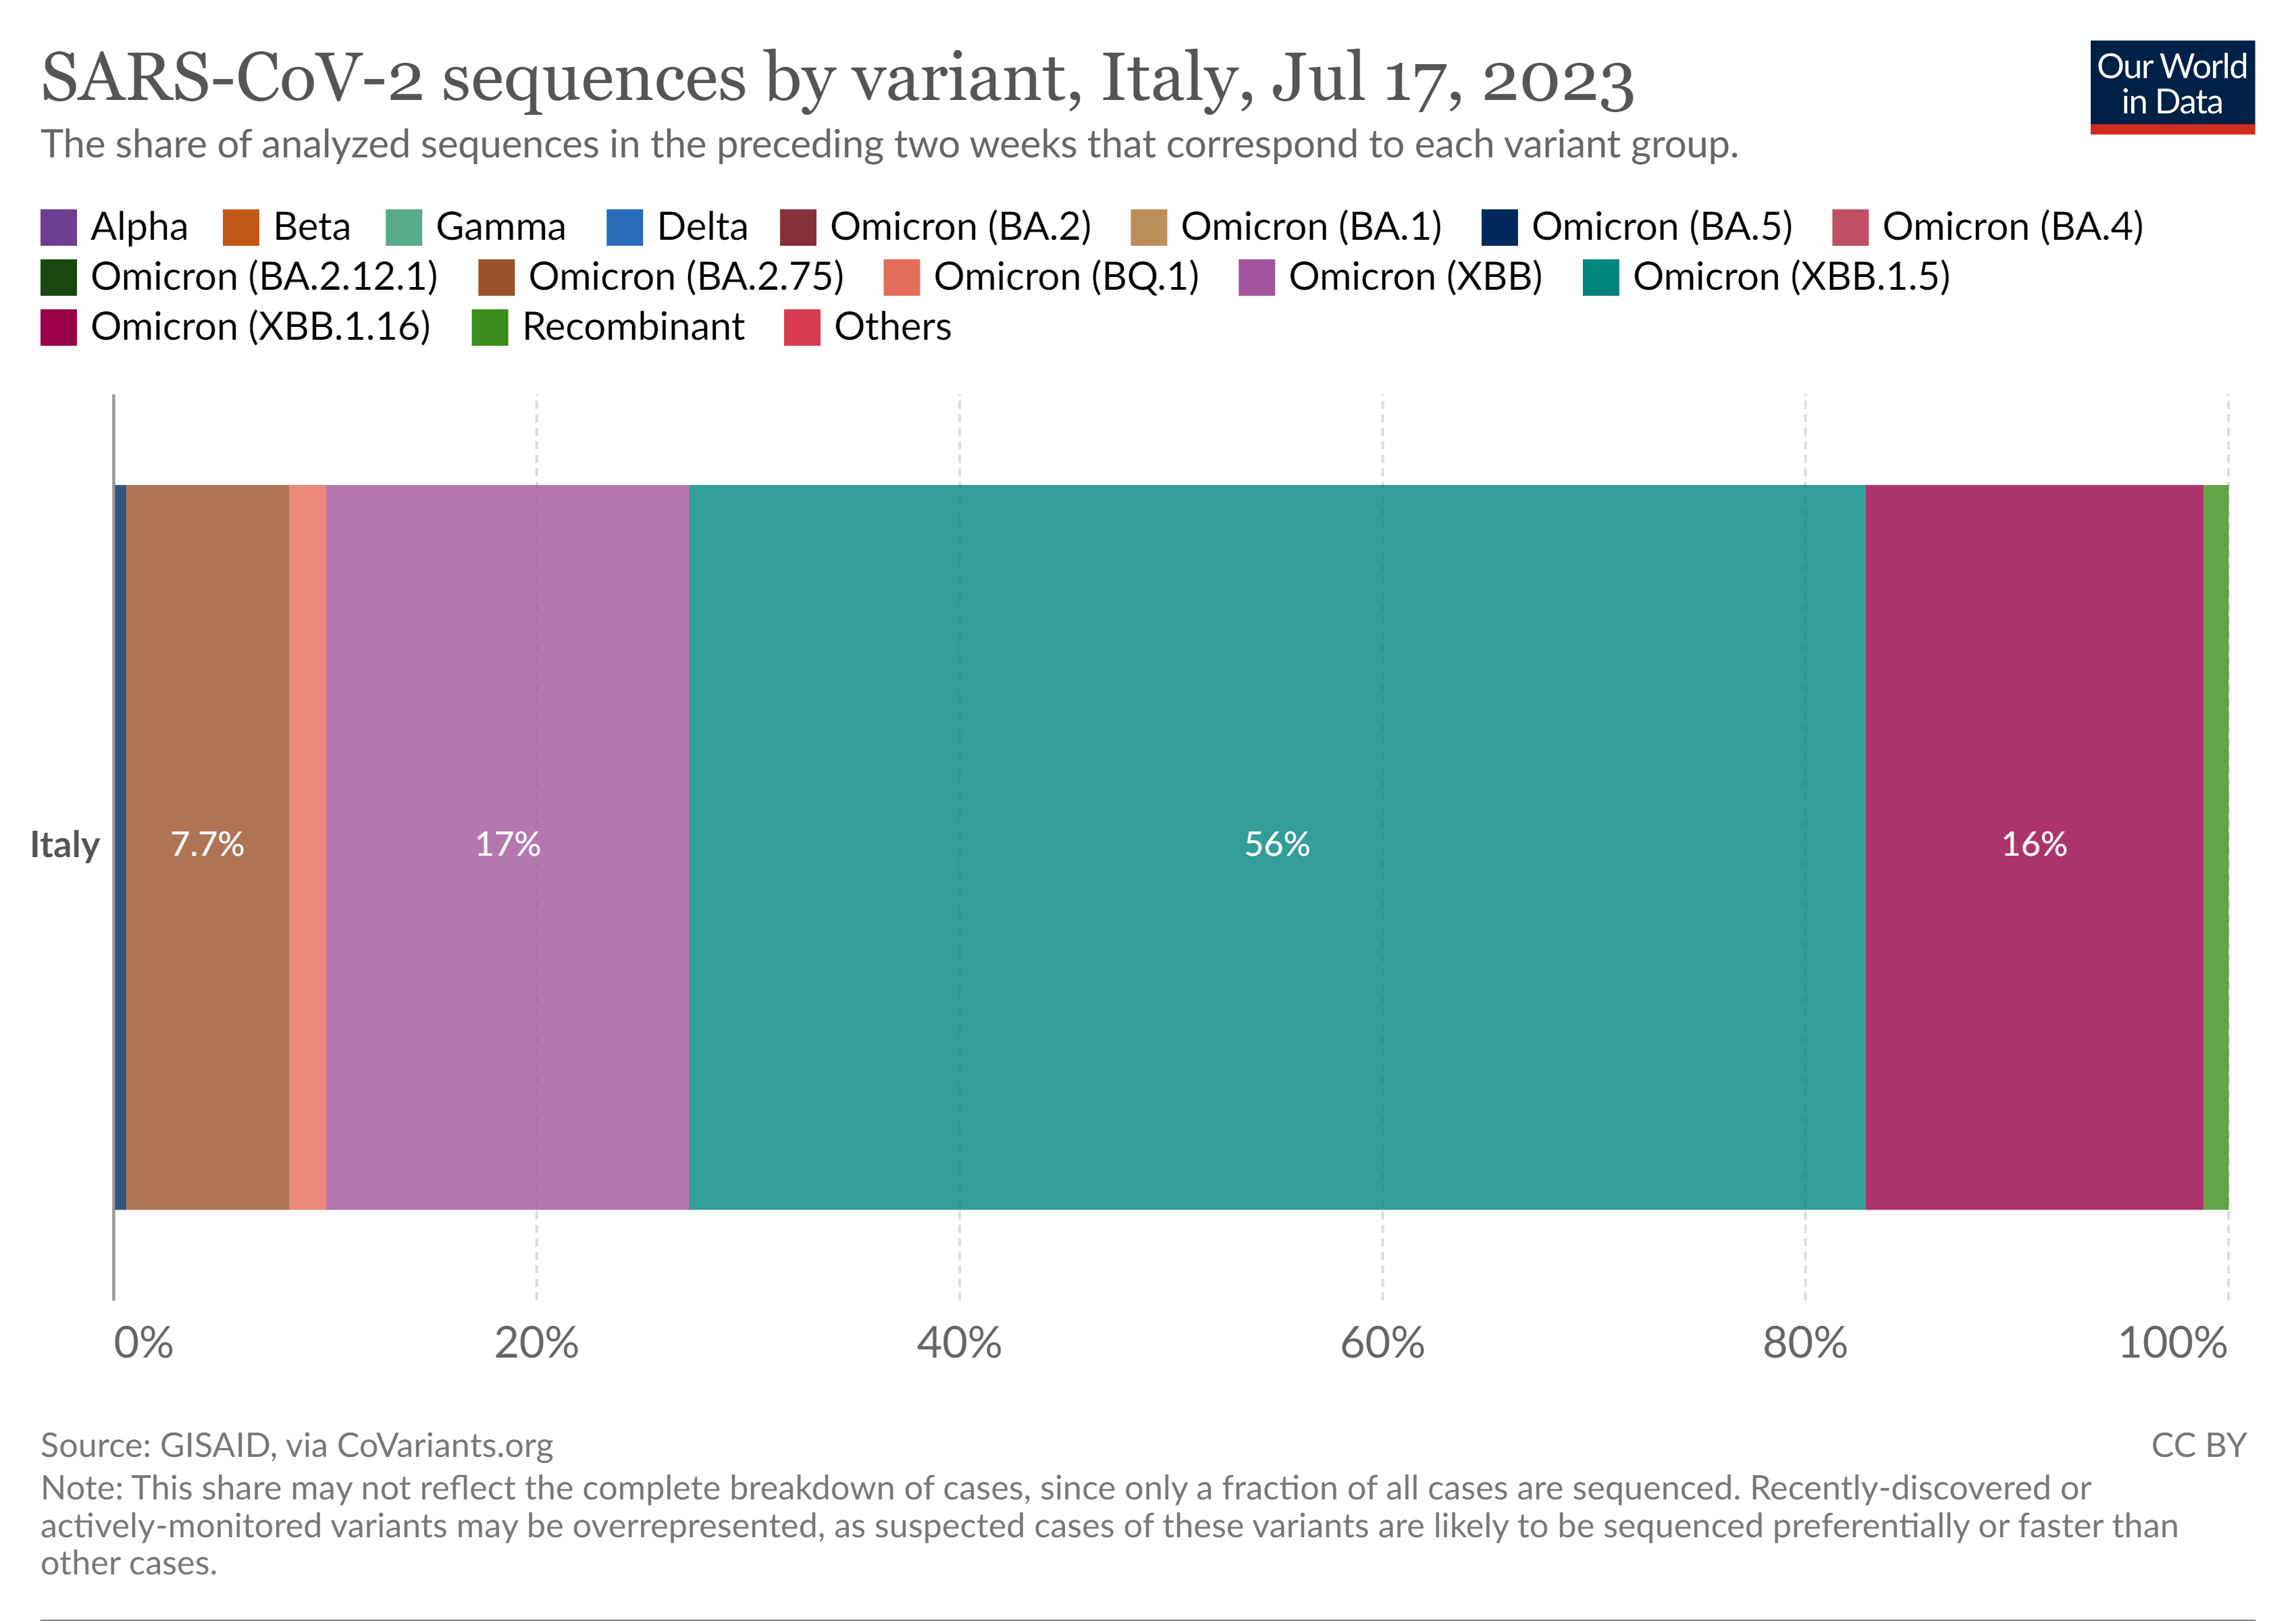
\includegraphics[width=\textwidth]{img/coronavirus-data-explorer.png}
	\captionof{figure}{Grafico delle mutazioni del virus SARS-COV2 preso da Our World in Data}
	\label{fig:covid_mutation}
\end{minipage}

Infine si nota come, seppur la definizione della funzione associata alla creazione di una
nuova \emph{Variant of Concern (VOC)} \ref{fig:voc} sia semplicistica e irrealistica, 
il grafico mostra come su un periodo di circa 3 anni, associabile alla durata del periodo covid, 
il numero di VOC sia pressoche' sovrapponibile con quanto osservato dai dati raccolti durante la pandemia \ref{fig:covid_mutation}. 

\subsection{Intervento non farmaceutico}
Il seguente grafico \ref{fig:abm_intervent} mostra l'andamento delle curve del modello
quando questo viene eseguito tramite l'applicazione di una qualche tipologia di intervento non farmaceutico. 
Le contromisure sono rappresentate come un insieme di valori appartenenti all'intervallo $[0, 1)$ 
le quali rappresentano cumulativamente un insieme di metriche differenti non esplicite che vanno a definire 
un insieme di misure di controllo. Le misure di controllo cercano di mimicare quelle associate al progetto 
\textbf{OxCGRT} il quale ha lo scopo di misurare la durezza delle contomisure applicate in un determinato paese; 
questo valore e' composito di 9 metriche: chiusura delle scuole; chiusura dei luoghi di lavoro; 
cancellazione di eventi pubblici; restrizioni agli assembramenti pubblici; 
chiusura dei trasporti pubblici; obbligo di rimanere a casa; campagne di informazione pubblica; 
restrizioni agli spostamenti interni e controlli sui viaggi internazionali.

\begin{minipage}{\linewidth}
	\centering
	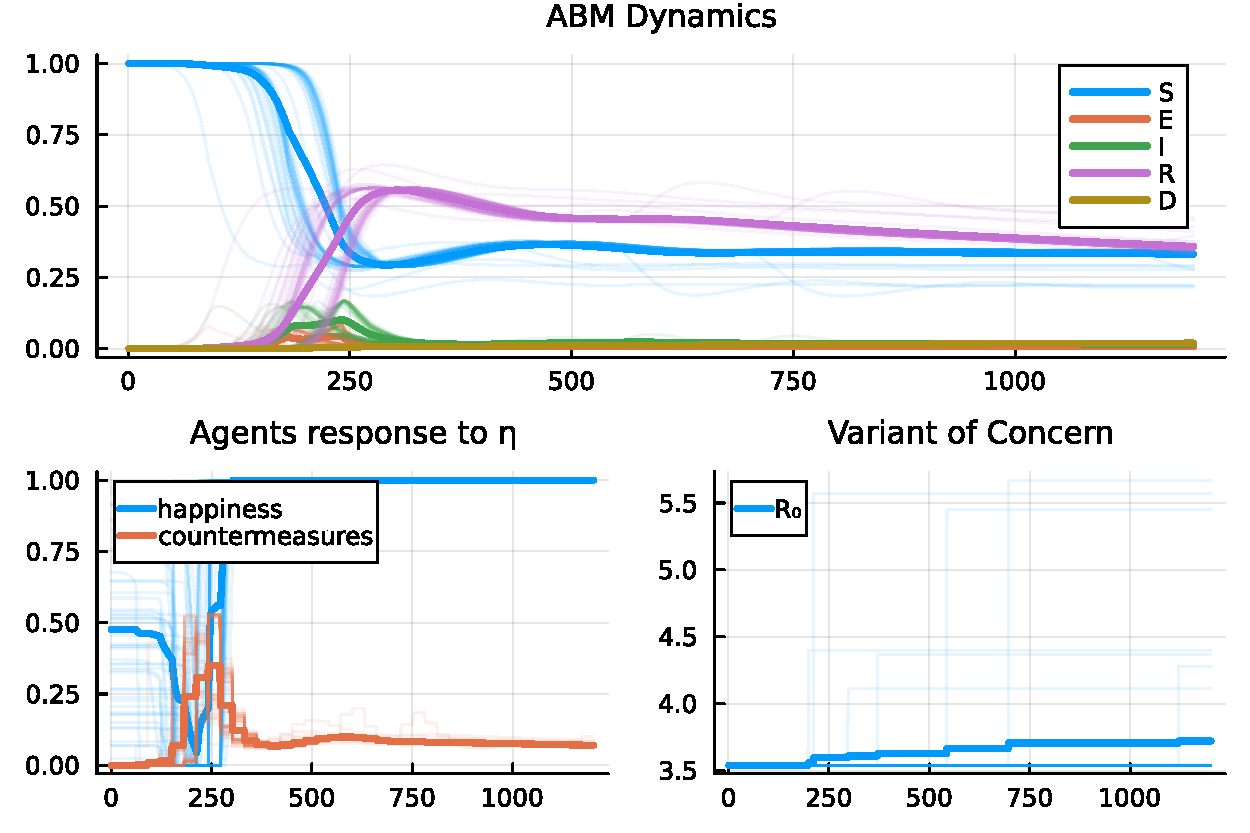
\includegraphics[width=\textwidth]{img/SocialNetworkABM_CONTROL.pdf}
	\captionof{figure}{Grafico cumulativo del modello con intervento non farmaceutico del controllore}
	\label{fig:abm_intervent}
\end{minipage}

Queste metriche sono metriche reali ma che nel modello vengono viste come un insieme unico, associabile 
ad una somma di medie dei valori di ogni metrica. Questa scelta porta a non avere un indice molto chiaro
ma permette comunque di avere un idea generale estremamente immediata dell'effetto che queste hanno sul modello.

Si nota come con l'applicazione di un insieme di contromisure, piu' o meno stringenti a seconda del periodo osservato, 
possiamo osservare come le curve epidemiologiche tendono ad appiattirsi, soprattutto quelle associate ai compartimenti 
\textbf{E, I}, le quali influenzano le curve \textbf{S, R}. In questo caso la ciclicita' del modello viene meno. 

Altro dato interessante e' il numero di VOC che e' diminuito rispetto al modello senza intervento.
Questo dipende generalmente dal comportamento delle contromisure. Infatti queste quando vengono applicate, 
oltre a influenzare il parametro \textbf{happiness}, vanno ad influenzare anche la matrice di flusso \ref{fig:migration matrix}
andando a ridurne i valori presenti. Questo fa si che oltre a dilazionare la diffusione della pandemia, 
va a dilazionare il comportamento della funzione che si occupa di generare una VOC \ref{fig:voc}. 

Questa infatti puo' attivarse sse nel nodo sono presenti individui infetti, in quanto non e' stata modellata la 
possibilita' che spontaneamente una nuova variante arrivi in un nuovo nodo senza un veicolo umano. Percio' 
applicare delle contromisure permette anche a contenere la diffusione di VOC nella popolazione osservata.

Si puo' osservare come la variabile di controllo \textbf{happiness} segua molto attentamente l'andamento sia delle 
contromisure che della pandemia, arrivando all'inizio della pandemia quando le contromisure sono piu' stringenti 
a diventare pressoche nulla. Successivamente, pur mantenendo un livello di contromisure sostenuto, la media
del valore di controllo tende ad alzarsi, seguendo il valore del compartimento \textbf{R}. Questo approccio sembra 
imitare il generale andamento della risposta che la popolazione italiana ha avuto alle prime misure di contenimento 
applicate realmente durante la pandemia da COVID-19.

\subsection{Intervento farmaceutico}
Il seguente grafico \ref{fig:abm_vaccine} mostra l'andamento delle curve del modello
quando questo viene eseguito tramite l'applicazione di una qualche tipologia di intervento farmaceutico.
Questo grafico dipende enormemente da quando viene trovato e successivamente applicato un intervento 
farmaceutico alla popolazione. Prima viene applicato un intervento farmaceutico piu' le curve si modificano 
e sono differenti dalll'andamento senza intervento \ref{fig:abm_no_intervent}, mentre piu' tempo passa piu'
il comportamento tende ad assomigliarsi.

\begin{minipage}{\linewidth}
	\centering
	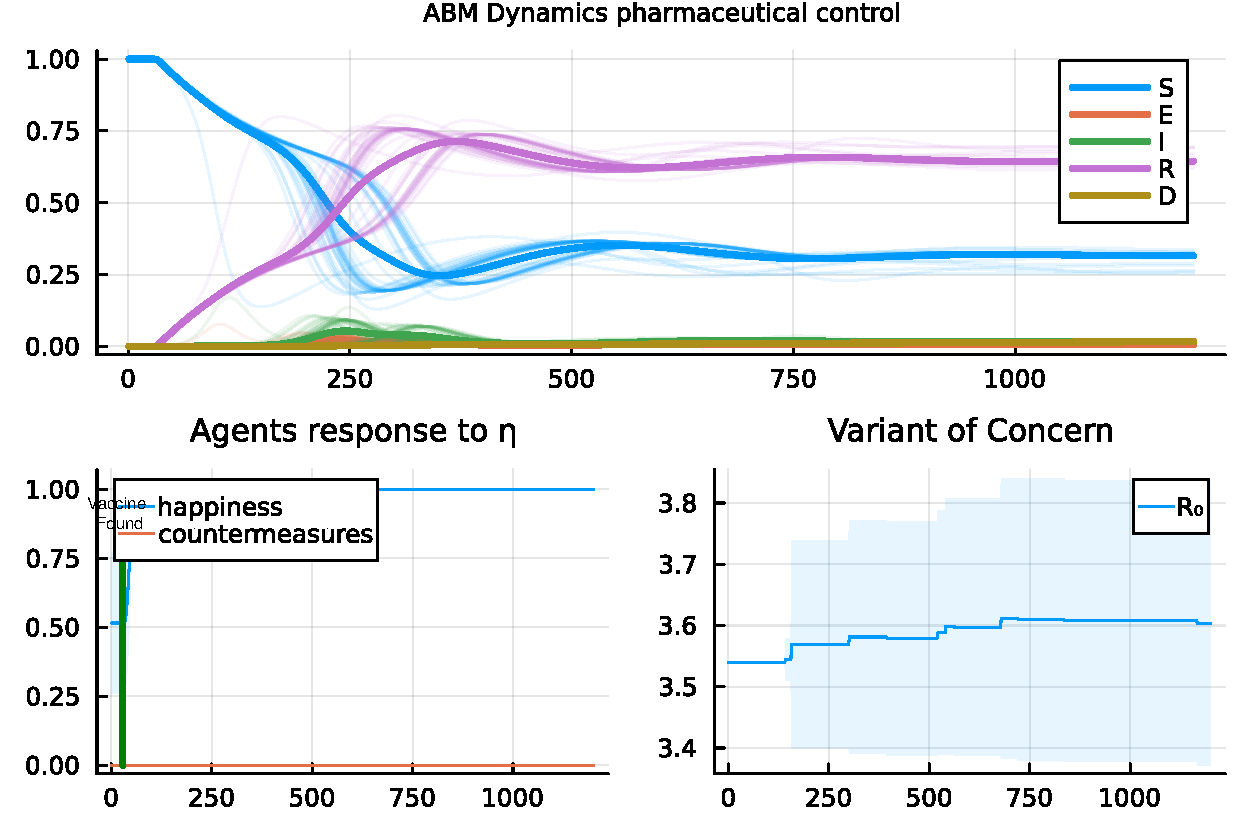
\includegraphics[width=\textwidth]{img/SocialNetworkABM_VACCINE.pdf}
	\captionof{figure}{Grafico cumulativo del modello con intervento del controllore tramite interventi farmaceutici come ad esempio un vaccino}
	\label{fig:abm_vaccine}
\end{minipage}

Il grafico mostra come se disponibili e applicate repentinamente, l'utilizzo di contromisure farmaceutiche permette 
permette di ridurre repentinamente le curve senza andare ad intaccare la curva di happiness in maniera troppo sensibile.

\subsection{Intervento farmaceutico e non farmaceutico}
Il seguente grafico \ref{fig:abm_all} mostra l'andamento delle curve del modello
quando questo viene eseguito tramite l'applicazione sia di un intervento di tipo farmaceutico 
come ad esempio l'utillizo di un vaccino, che di contromisure non farmaceutiche.

\begin{minipage}{\linewidth}
	\centering
	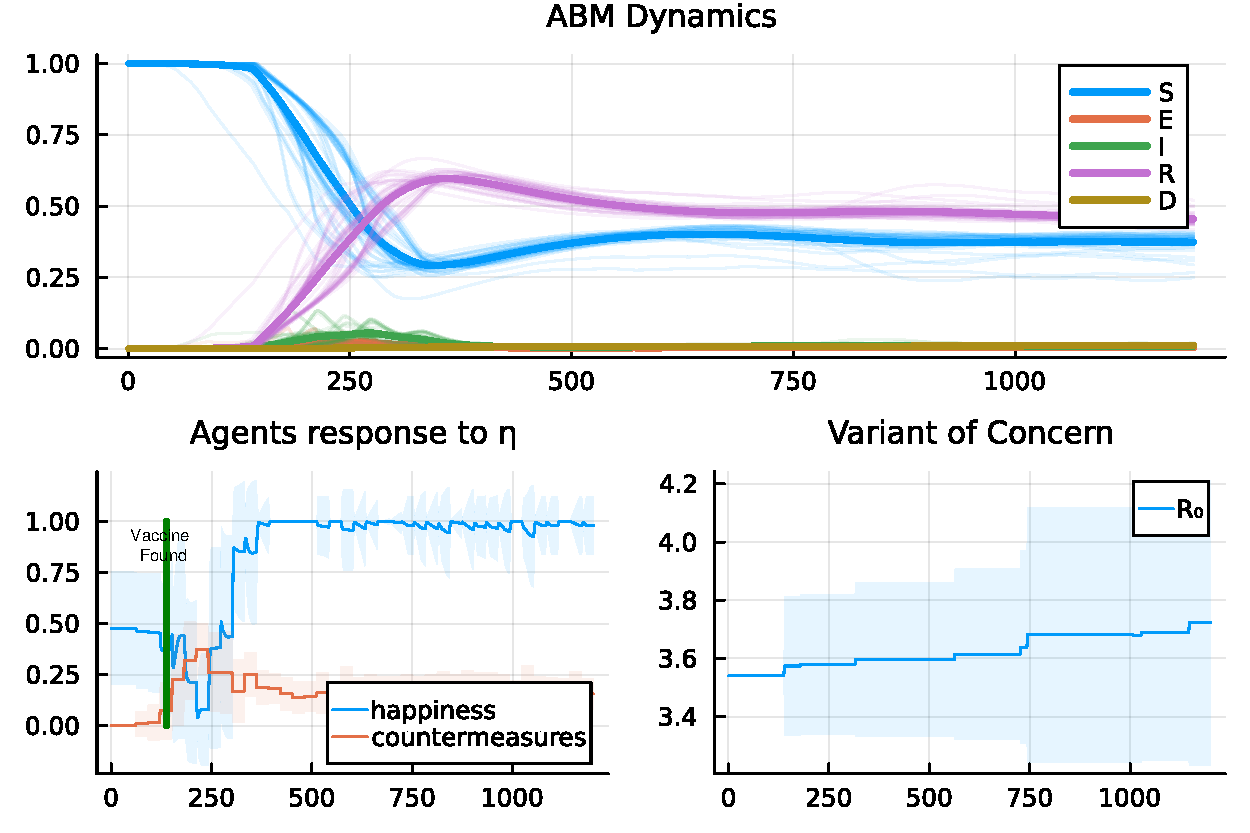
\includegraphics[width=\textwidth]{img/SocialNetworkABM_ALL.pdf}
	\captionof{figure}{Grafico cumulativo del modello con intervento del controllore tramite vaccino e metodi di prevenzione non farmaceutici}
	\label{fig:abm_all}
\end{minipage}

In questo caso viene mostrato l'andamento delle curve tenendo in considerazione l'utilizzo di ogni mezzo
per prevenire e contrastare l'epidemia. L'uitilizzo combinato di mezzi farmaceutici e non permettono 
si appiattire notevolmente la curva di infetti andando a creare velocemente un immunita' di gruppo 
che rende la popolazione meno suscettibile alle varianti. Questo inoltre fa si che la \emph{happiness} media
del modello sia generalmente piu' alta anche quando vengono applicate delle contromisure che vanno ad 
intaccare la felicita' della popolazione (ad esempio un lockdown). 

Queste contromisure non farmaceutiche sono in genere meno stringenti e meno prolungate, permettendo quindi
alla popolazione di non avere un calo drastico della happiness generale come in figura \ref{fig:abm_intervent}.
Tuttavia dipendono fortemente da quando le contromisure farmaceutiche (il vaccino) vengono applicate
e con che efficacia questo riesce ad entrare in circolazione. 

Tuttavia questo dimostra come l'utilizzo di un vaccino a priori sia un metodo molto efficace per contrastare
una epidemia, e che ovviamente l'efficacia di questo dipenda molto e soprattutto da quando viene applicato 
alla popolazione. Successivamente si puo' notare come le misure non farmaceutiche di prevenzione e contrasto
dell'epidemia sono un mezzo efficace per controllare la diffusione dell'infezione, ma queste hanno un costo 
in termini sia di generale qualita' della vita, che anche economico, non indifferente come mostrato dai grafici 
precedenti e dall'esperienza diretta che si e' avuto con la pandemia da COVID-19. 

\subsection{Analisi di sensitività}
\begin{minipage}{\linewidth}
	\centering
	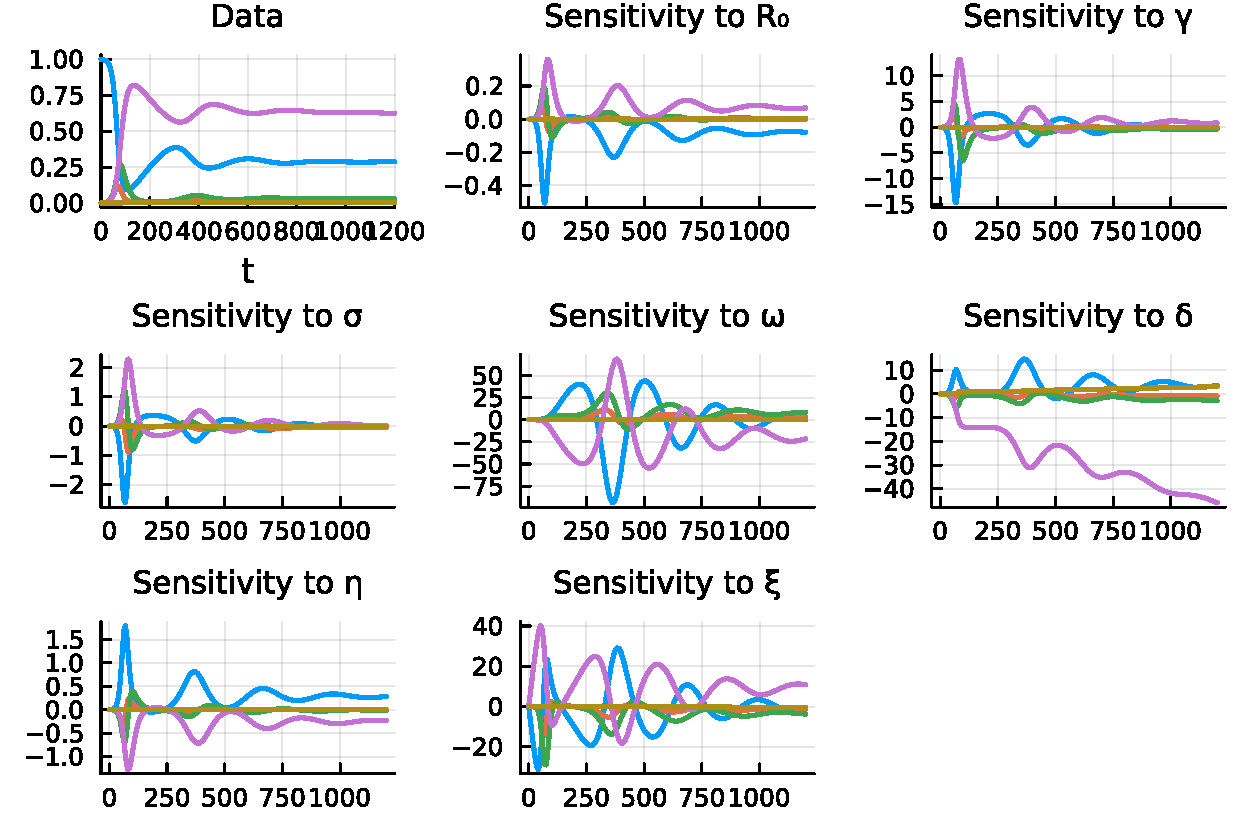
\includegraphics[width=\textwidth]{img/sa.pdf}
	\captionof{figure}{Grafico rappresentante l'analisi di sensitivita' del modello}
	\label{fig:sens_anal}
\end{minipage}